\documentclass[12pt,a4paper]{article}
\usepackage[margin=2cm]{geometry}
\usepackage{xeCJK}
\usepackage{fontspec}
\setCJKmainfont{Noto Serif CJK TC}[Script=CJK]
\usepackage{amsmath,amssymb}
\usepackage{graphicx}
\usepackage{fancyhdr}
\setlength{\headheight}{14.5pt}
\addtolength{\topmargin}{-2.5pt}
\usepackage{hyperref}
\usepackage{listings}
\usepackage{enumitem}
\usepackage{titlesec}
\usepackage{caption}
\usepackage{indentfirst}
\usepackage{booktabs}
\usepackage{longtable}
\usepackage{multirow}
\usepackage{array}
\usepackage{tabularx}
\usepackage{float}
\usepackage{minted}
\usepackage{tikz}
\usepackage{pgffor} % for loop
\usetikzlibrary{positioning,arrows.meta}
\usepackage{subcaption} % for subfigure environment

\setlength{\parindent}{2em}
\pagestyle{fancy}
\fancyhf{}
\cfoot{\thepage}
\linespread{1.3}
\setminted{
    linenos,                % 行號
    frame=lines,            % 上下框線
    framesep=5pt,           % 程式碼與邊框距離
    numbersep=8pt,          % 行號與程式碼距離
    fontsize=\scriptsize,   % 字體大小
    breaklines,             % 自動換行
    tabsize=4,              % tab 寬度
    rulecolor=\color{black},% 框線顏色
    xleftmargin=1.5em       % 左側縮排
}

\title{Fundamentals of Biomedical Image Processing HW 1}
\author{B12508026戴偉璿}
\date{\today}


\begin{document}

\maketitle
\lhead{Fundamentals of Biomedical Image Processing Homework 1}
\rhead{B12508026戴偉璿}

\section{Theorem questions}
\begin{enumerate}
    \item
    \begin{enumerate}
        \item The picture size is $1024\times 1024$ pixels, and each pixel contains 256 intensity levels(8 bits,i.e., 1 byte). Therefore, the total data size is $1024\times 1024 \times 1 = 1,048,576$ bytes. Since each packet requires 10 bits to transmit 1 byte of data, the total number of bits to be transmitted is 10,485,760 bits. With the baud rate of 56k, the transmission time is $10,485,760\div 56000 \approx 187.25(sec)\approx 3.12$ minutes.
        \item With the baud rate of 3000k, the transmission time is\\ $10,485,760\div 3,000,000 \approx 3.495(sec)\approx 0.058$ minutes.
    \end{enumerate}
    \item $V=\{1 ,2\}$, so the graph would be Fig.~\ref{fig:2a}:
    \begin{figure}[H]
        \centering
        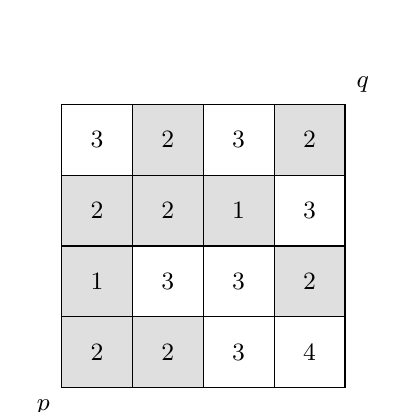
\begin{tikzpicture}[scale=0.9, every node/.style={font=\small}][H]
  %----- 基本參數 -----
  \def\cell#1#2#3{ % (row, col, value)
    % 座標:左下(1,1),右上(4,4);但我們用 top-down 排列所以要轉換
    \pgfmathsetmacro{\x}{#2-1}
    \pgfmathsetmacro{\y}{4-#1}
    % 填色:V={1,2} 可走(light gray),其他白色
    \ifnum#3<3
      \fill[gray!25] (\x,\y) rectangle ++(1,1);
    \else
      \fill[white]   (\x,\y) rectangle ++(1,1);
    \fi
    % 外框
    \draw (\x,\y) rectangle ++(1,1);
    % 數字
    \node at (\x+0.5,\y+0.5) {\small #3};
  }
  %----- 填資料(row, col, value) -----
  % Row 1 (top): 3 2 3 2(q)
  \cell{1}{1}{3}  \cell{1}{2}{2}  \cell{1}{3}{3}  \cell{1}{4}{2}
  % Row 2: 2 2 1 3
  \cell{2}{1}{2}  \cell{2}{2}{2}  \cell{2}{3}{1}  \cell{2}{4}{3}
  % Row 3: 1 3 3 2
  \cell{3}{1}{1}  \cell{3}{2}{3}  \cell{3}{3}{3}  \cell{3}{4}{2}
  % Row 4 (bottom): 2(p) 2 3 4
  \cell{4}{1}{2}  \cell{4}{2}{2}  \cell{4}{3}{3}  \cell{4}{4}{4}

  %----- 標記 p 與 q -----
  % p at (row=4,col=1) -> (x=0,y=0)
  \node[below left=1pt] at (0,0) {$p$};
  % q at (row=1,col=4) -> (x=3,y=3)
  \node[above right=1pt] at (4,4) {$q$};

%   %----- shortest-8(藍色,長度 4): p(4,1)->(3,1)->(2,2)->(2,3)->q(1,4) -----
%   \draw[very thick,blue,-{Stealth[length=3mm]}]
%     (0.5,0.5) -- (0.5,1.5) -- (1.5,2.5) -- (2.5,2.5) -- (3.5,3.5);

%   %----- shortest-m(橙色,長度 5): p->(3,1)->(2,1)->(2,2)->(2,3)->q -----
%   \draw[very thick,orange!90!black,-{Stealth[length=3mm]}]
%     (0.5,0.5) -- (0.5,1.5) -- (0.5,2.5) -- (1.5,2.5) -- (2.5,2.5) -- (3.5,3.5);

%   %----- 圖例 -----
%   \draw[very thick,blue]   (0.1,-0.7)--+(0.6,0) node[right,black]{shortest-8 length $=4$};
%   \draw[very thick,orange!90!black] (2.6,-0.7)--+(0.6,0) node[right,black]{shortest-m length $=5$};
%   \node[black] at (2,-1.2) {shortest-4: no 4-connected path (q is 4-blocked)};
\end{tikzpicture}
        \caption{The grid graph with $V=\{1,2\}$ (gray cells are passable)}
        \label{fig:2a}
    \end{figure}
    \newpage
    \begin{enumerate}
        \item \fbox{shortest-4}: Only up, down, left, right movements are allowed. So the path would be:
        \begin{figure}[H]
            \centering
            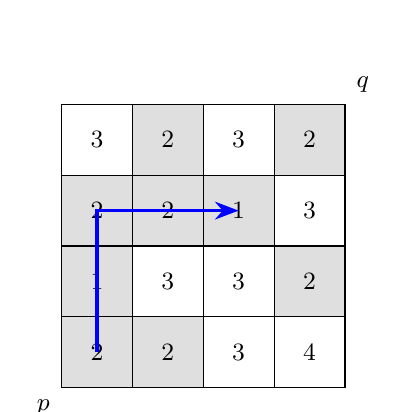
\begin{tikzpicture}[scale=0.9, every node/.style={font=\small}][H]
  %----- 基本參數 -----
  \def\cell#1#2#3{ % (row, col, value)
    % 座標:左下(1,1),右上(4,4);但我們用 top-down 排列所以要轉換
    \pgfmathsetmacro{\x}{#2-1}
    \pgfmathsetmacro{\y}{4-#1}
    % 填色:V={1,2} 可走(light gray),其他白色
    \ifnum#3<3
      \fill[gray!25] (\x,\y) rectangle ++(1,1);
    \else
      \fill[white]   (\x,\y) rectangle ++(1,1);
    \fi
    % 外框
    \draw (\x,\y) rectangle ++(1,1);
    % 數字
    \node at (\x+0.5,\y+0.5) {\small #3};
  }
  %----- 填資料(row, col, value) -----
  % Row 1 (top): 3 2 3 2(q)
  \cell{1}{1}{3}  \cell{1}{2}{2}  \cell{1}{3}{3}  \cell{1}{4}{2}
  % Row 2: 2 2 1 3
  \cell{2}{1}{2}  \cell{2}{2}{2}  \cell{2}{3}{1}  \cell{2}{4}{3}
  % Row 3: 1 3 3 2
  \cell{3}{1}{1}  \cell{3}{2}{3}  \cell{3}{3}{3}  \cell{3}{4}{2}
  % Row 4 (bottom): 2(p) 2 3 4
  \cell{4}{1}{2}  \cell{4}{2}{2}  \cell{4}{3}{3}  \cell{4}{4}{4}

  %----- 標記 p 與 q -----
  % p at (row=4,col=1) -> (x=0,y=0)
  \node[below left=1pt] at (0,0) {$p$};
  % q at (row=1,col=4) -> (x=3,y=3)
  \node[above right=1pt] at (4,4) {$q$};

  %----- shortest-8(藍色,長度 4): p(4,1)->(3,1)->(2,2)->(2,3)->q(1,4) -----
  \draw[very thick,blue,-{Stealth[length=3mm]}]
    (0.5,0.5) -- (0.5,1.5) -- (0.5,2.5) -- (1.5,2.5) -- (2.5,2.5) ;

%   %----- shortest-m(橙色,長度 5): p->(3,1)->(2,1)->(2,2)->(2,3)->q -----
%   \draw[very thick,orange!90!black,-{Stealth[length=3mm]}]
%     (0.5,0.5) -- (0.5,1.5) -- (0.5,2.5) -- (1.5,2.5) -- (2.5,2.5) -- (3.5,3.5);

%   %----- 圖例 -----
%   \draw[very thick,blue]   (0.1,-0.7)--+(0.6,0) node[right,black]{shortest-8 length $=4$};
%   \draw[very thick,orange!90!black] (2.6,-0.7)--+(0.6,0) node[right,black]{shortest-m length $=5$};
%   \node[black] at (2,-1.2) {shortest-4: no 4-connected path (q is 4-blocked)};
\end{tikzpicture}
            \caption{No 4-connected path (q is 4-blocked)}
            \label{fig:2a_s4}
        \end{figure}
        As the Fig.~\ref{fig:2a_s4} shows, there's no path from last step $(3, 3)$ to node $q(4, 4)$, so the length is \textbf{infinity}.
        \item \fbox{shortest-8}: Up, down, left, right, and diagonal movements are allowed. So the path would be:
        \begin{figure}[H]
            \centering
            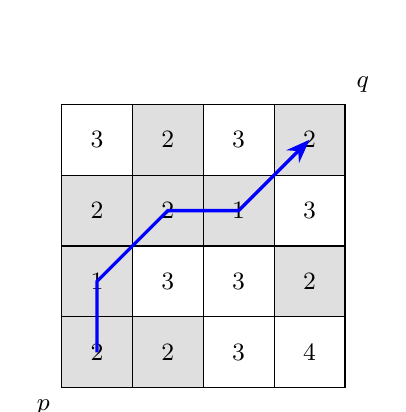
\begin{tikzpicture}[scale=0.9, every node/.style={font=\small}][H]
  %----- 基本參數 -----
  \def\cell#1#2#3{ % (row, col, value)
    % 座標:左下(1,1),右上(4,4);但我們用 top-down 排列所以要轉換
    \pgfmathsetmacro{\x}{#2-1}
    \pgfmathsetmacro{\y}{4-#1}
    % 填色:V={1,2} 可走(light gray),其他白色
    \ifnum#3<3
      \fill[gray!25] (\x,\y) rectangle ++(1,1);
    \else
      \fill[white]   (\x,\y) rectangle ++(1,1);
    \fi
    % 外框
    \draw (\x,\y) rectangle ++(1,1);
    % 數字
    \node at (\x+0.5,\y+0.5) {\small #3};
  }
  %----- 填資料(row, col, value) -----
  % Row 1 (top): 3 2 3 2(q)
  \cell{1}{1}{3}  \cell{1}{2}{2}  \cell{1}{3}{3}  \cell{1}{4}{2}
  % Row 2: 2 2 1 3
  \cell{2}{1}{2}  \cell{2}{2}{2}  \cell{2}{3}{1}  \cell{2}{4}{3}
  % Row 3: 1 3 3 2
  \cell{3}{1}{1}  \cell{3}{2}{3}  \cell{3}{3}{3}  \cell{3}{4}{2}
  % Row 4 (bottom): 2(p) 2 3 4
  \cell{4}{1}{2}  \cell{4}{2}{2}  \cell{4}{3}{3}  \cell{4}{4}{4}

  %----- 標記 p 與 q -----
  % p at (row=4,col=1) -> (x=0,y=0)
  \node[below left=1pt] at (0,0) {$p$};
  % q at (row=1,col=4) -> (x=3,y=3)
  \node[above right=1pt] at (4,4) {$q$};

  %----- shortest-8(藍色,長度 4): p(4,1)->(3,1)->(2,2)->(2,3)->q(1,4) -----
  \draw[very thick,blue,-{Stealth[length=3mm]}]
    (0.5,0.5) -- (0.5,1.5) -- (1.5,2.5) -- (2.5,2.5) -- (3.5,3.5);

%   %----- shortest-m(橙色,長度 5): p->(3,1)->(2,1)->(2,2)->(2,3)->q -----
%   \draw[very thick,orange!90!black,-{Stealth[length=3mm]}]
%     (0.5,0.5) -- (0.5,1.5) -- (0.5,2.5) -- (1.5,2.5) -- (2.5,2.5) -- (3.5,3.5);

%   %----- 圖例 -----
%   \draw[very thick,blue]   (0.1,-0.7)--+(0.6,0) node[right,black]{shortest-8 length $=4$};
%   \draw[very thick,orange!90!black] (2.6,-0.7)--+(0.6,0) node[right,black]{shortest-m length $=5$};
%   \node[black] at (2,-1.2) {shortest-4: no 4-connected path (q is 4-blocked)};
\end{tikzpicture}
            \caption{shortest-8 path (length = 4)}
            \label{fig:2a_s8}
        \end{figure}
        As the Fig.~\ref{fig:2a_s8} shows, it takes 4 steps to reach from $p(1, 1)$ to $q(4, 4)$,\\ so the length is \textbf{4}.
        \newpage
        \item \fbox{shortest-m}: The path can only move to the 8-neighbors with the minimum value. So the path would be:
        \begin{figure}[H]
            \centering
            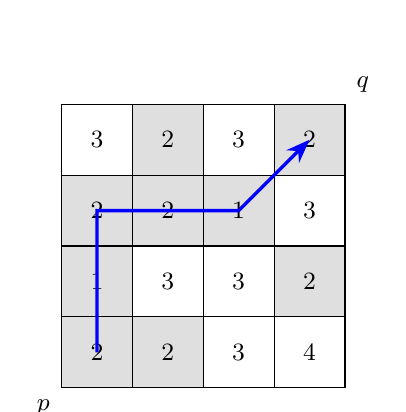
\begin{tikzpicture}[scale=0.9, every node/.style={font=\small}][H]
  %----- 基本參數 -----
  \def\cell#1#2#3{ % (row, col, value)
    % 座標:左下(1,1),右上(4,4);但我們用 top-down 排列所以要轉換
    \pgfmathsetmacro{\x}{#2-1}
    \pgfmathsetmacro{\y}{4-#1}
    % 填色:V={1,2} 可走(light gray),其他白色
    \ifnum#3<3
      \fill[gray!25] (\x,\y) rectangle ++(1,1);
    \else
      \fill[white]   (\x,\y) rectangle ++(1,1);
    \fi
    % 外框
    \draw (\x,\y) rectangle ++(1,1);
    % 數字
    \node at (\x+0.5,\y+0.5) {\small #3};
  }
  %----- 填資料(row, col, value) -----
  % Row 1 (top): 3 2 3 2(q)
  \cell{1}{1}{3}  \cell{1}{2}{2}  \cell{1}{3}{3}  \cell{1}{4}{2}
  % Row 2: 2 2 1 3
  \cell{2}{1}{2}  \cell{2}{2}{2}  \cell{2}{3}{1}  \cell{2}{4}{3}
  % Row 3: 1 3 3 2
  \cell{3}{1}{1}  \cell{3}{2}{3}  \cell{3}{3}{3}  \cell{3}{4}{2}
  % Row 4 (bottom): 2(p) 2 3 4
  \cell{4}{1}{2}  \cell{4}{2}{2}  \cell{4}{3}{3}  \cell{4}{4}{4}

  %----- 標記 p 與 q -----
  % p at (row=4,col=1) -> (x=0,y=0)
  \node[below left=1pt] at (0,0) {$p$};
  % q at (row=1,col=4) -> (x=3,y=3)
  \node[above right=1pt] at (4,4) {$q$};

  %----- shortest-8(藍色,長度 4): p(4,1)->(3,1)->(2,2)->(2,3)->q(1,4) -----
  \draw[very thick,blue,-{Stealth[length=3mm]}]
    (0.5,0.5) -- (0.5,1.5) -- (0.5,2.5) -- (1.5,2.5) -- (2.5,2.5) -- (3.5,3.5);

%   %----- shortest-m(橙色,長度 5): p->(3,1)->(2,1)->(2,2)->(2,3)->q -----
%   \draw[very thick,orange!90!black,-{Stealth[length=3mm]}]
%     (0.5,0.5) -- (0.5,1.5) -- (0.5,2.5) -- (1.5,2.5) -- (2.5,2.5) -- (3.5,3.5);

%   %----- 圖例 -----
%   \draw[very thick,blue]   (0.1,-0.7)--+(0.6,0) node[right,black]{shortest-8 length $=4$};
%   \draw[very thick,orange!90!black] (2.6,-0.7)--+(0.6,0) node[right,black]{shortest-m length $=5$};
%   \node[black] at (2,-1.2) {shortest-4: no 4-connected path (q is 4-blocked)};
\end{tikzpicture}
            \caption{shortest-m path (length = 5)}
            \label{fig:2a_sm}
        \end{figure}
        As the Fig.~\ref{fig:2a_sm} shows, it takes 5 steps to reach from $p(1, 1)$ to $q(4, 4)$,\\ so the length is \textbf{5}.
    \end{enumerate}
\end{enumerate}

\newpage
\section{Programming exercises}

All code can be found at \url{https://github.com/W-X-Dai/tex/tree/main/imgProc/HW1/code}.

\begin{enumerate}
    \item To draw a triangle, we can find its three vertices, and then use the line-drawing algorithm to connect them. The result is Fig.~\ref{fig:p1}:
    \begin{figure}[H]
        \centering
        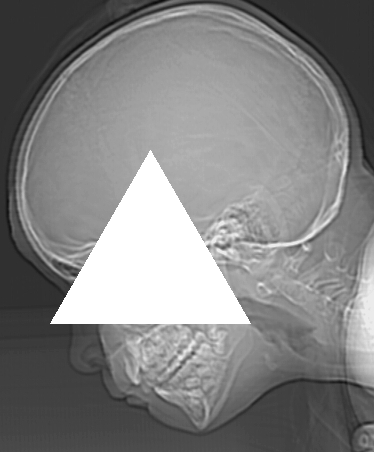
\includegraphics[width=0.2\textwidth]{src/img/p1/output.png}
        \caption{The result of drawing an equilateral triangle}
        \label{fig:p1}
    \end{figure}
    Following is the code: 
    \begin{minted}{python}
import os
import cv2
import numpy as np

os.makedirs("result/p1", exist_ok=True)

img = cv2.imread("src/Fig1.bmp", cv2.IMREAD_GRAYSCALE)
if img is None:
    print("Error: Unable to load image.")
    exit()

"""Calculating the vertices coordinates of an equilateral triangle."""
top = (150, 150)
h = int((3**0.5 / 2) * 200) 
left = (150 - 100, 150 + h)
right = (150 + 100, 150 + h)

pts = np.array([top, left, right], np.int32)

cv2.fillPoly(img, [pts], 255)

cv2.imwrite("result/p1/output.bmp", img)
print("Result image saved to result/p1/output.bmp")

cv2.imshow("Triangle", img)
cv2.waitKey(0)
cv2.destroyAllWindows()
    \end{minted}
    \newpage
    \item To transfer the gray levels of the original image to assigned levels, we can use the formula:
    $$\text{new\_pixel} \;=\; \left\lfloor \frac{\text{old\_pixel} \cdot \text{levels}}{256} \right\rfloor \cdot \frac{256}{\text{levels}} \;+\; \frac{128}{\text{levels}}$$
    The result is in Fig.~\ref{fig:p2}:
    \begin{figure}[H]
    \centering
    \foreach \n in {2, 4, 8, 16, 32, 64, 128, 256}{
        \begin{subfigure}{0.20\textwidth}
        \includegraphics[width=\linewidth]{src/img/p2/gray_\n.png}
        \caption{gray\_\n}
        \end{subfigure}
    }
    \caption{Gray images from 2 to 256 (256 is the original image)}
    \label{fig:p2}
    \end{figure}
    Following is the code:
    \begin{minted}{python}
import os
import cv2
import numpy as np

os.makedirs("result/p2", exist_ok=True)

def reduce_gray_levels(img, nLevels=2):
    if nLevels < 2 or nLevels > 256 or (nLevels & (nLevels - 1)):
        raise ValueError("invalid input: nLevels must be a power of 2 and between 2 and 256.")

    delta = 256 // nLevels
    quantized = (img // delta) * delta + delta // 2
    return quantized.astype(np.uint8)

img = cv2.imread("src/Fig1.bmp", cv2.IMREAD_GRAYSCALE)
if img is None:
    raise FileNotFoundError("Cannot open Fig1.bmp")

nLevels = int(input("Enter the number of gray levels (should be a power of 2 and between 2 and 256, e.g., 2,4,8,...,256): "))

out = reduce_gray_levels(img, nLevels)

cv2.imwrite(f"result/p2/gray_{nLevels}.bmp", out)
print(f"Result image saved to result/p2/gray_{nLevels}.bmp")

cv2.imshow(f"{nLevels} levels", out)
cv2.waitKey(0)
cv2.destroyAllWindows()
    \end{minted}
    \item To rotate the image by a specified angle, we can use the rotation matrix to calculate the new coordinates of each pixel. I once implemented a bilinear interpolation algorithm and then modified it into a nearest neighbor interpolation. The result is shown in Fig.~\ref{fig:p3}.

    \begin{figure}[H]
        \centering
        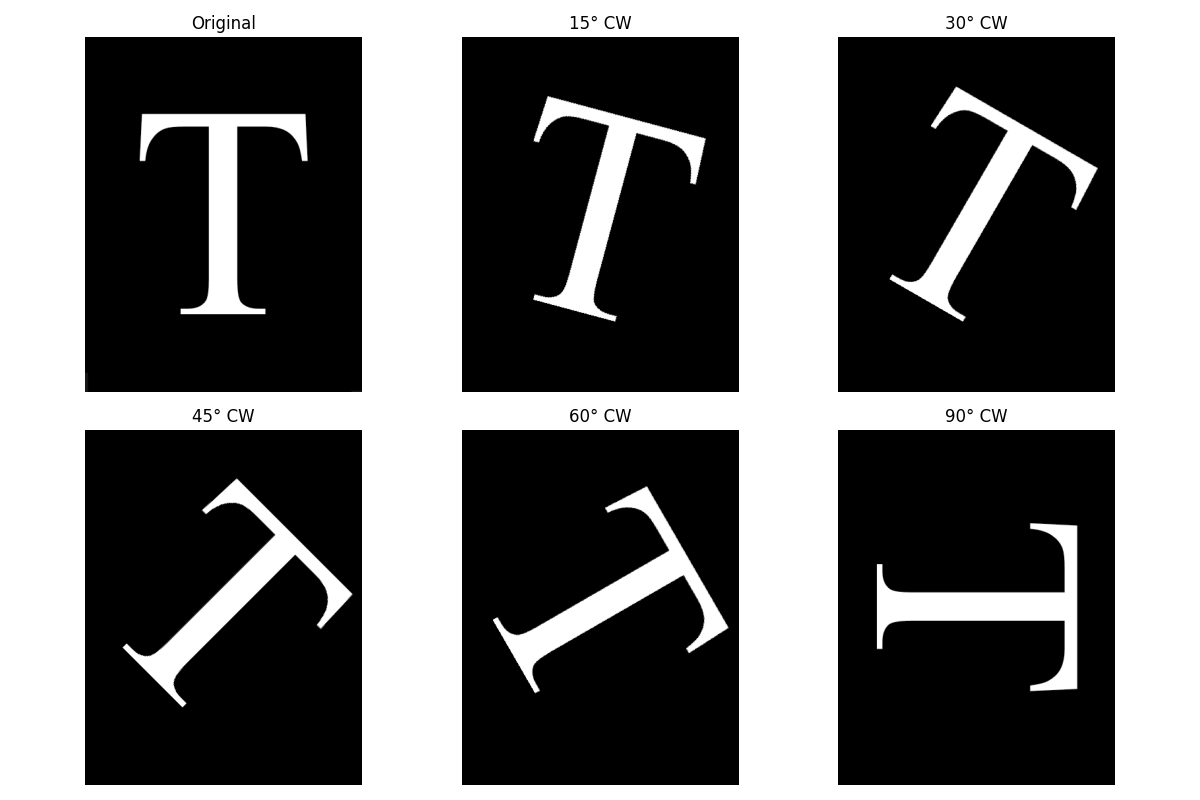
\includegraphics[width=1\textwidth]{src/img/p3/combined_grid.png}
        \caption{The result of rotation}
        \label{fig:p3}
    \end{figure}
    Following is the code:
    \begin{minted}{python}
import os
import cv2
import numpy as np
import math
import matplotlib.pyplot as plt

"""This is used to be a bilinear interpolation function I've finished in the past, but I changed to nearest neighbor interpolation for simplicity."""
def bi_affine(img, A):
    img_out = np.zeros_like(img)
    inv = np.linalg.inv(A)

    h, w = img.shape
    for i in range(h):          # row
        for j in range(w):      # col
            origin_T = np.array([[j], [i], [1]])
            inv_T = inv @ origin_T

            c, r = inv_T[0].item(), inv_T[1].item()

            # clamp
            r = min(max(r, 0), h-1)
            c = min(max(c, 0), w-1)

            # nearest neighbor
            r_nn, c_nn = int(round(r)), int(round(c))
            img_out[i, j] = img[r_nn, c_nn]

    return img_out

def get_rotation_matrix(h, w, angle_deg):
    cx, cy = w/2, h/2
    theta = math.radians(angle_deg)
    cos_t, sin_t = math.cos(theta), math.sin(theta)

    A = np.array([
        [ cos_t, sin_t, (1-cos_t)*cx-sin_t*cy],
        [-sin_t, cos_t, (1-cos_t)*cy+sin_t*cx],
        [     0,     0,                     1]
    ], dtype=np.float32)

    return A

if __name__ == '__main__':
    os.makedirs("result/p3", exist_ok=True)

    img = cv2.imread('src/Fig2.bmp', cv2.IMREAD_GRAYSCALE)
    if img is None:
        raise FileNotFoundError("Cannot find Fig2.bmp")
    
    h, w = img.shape

    angles = [15, 30, 45, 60, 90]
    results = [img]

    for angle in angles:
        """minus angle for clockwise rotation"""
        A = get_rotation_matrix(h, w, -angle)
        rotated = bi_affine(img, A)

        cv2.imwrite(f"result/p3/rot_{angle}.bmp", rotated)
        results.append(rotated)

    print("Result images saved to result/p3/")

    plt.figure(figsize=(12, 8))
    titles = ["Original"] + [f"{a}° CW" for a in angles]

    for idx, (title, im) in enumerate(zip(titles, results), 1):
        plt.subplot(2, 3, idx)
        plt.imshow(im, cmap="gray")
        plt.title(title)
        plt.axis("off")

    plt.tight_layout()
    plt.savefig("result/p3/combined_grid.png")
    plt.show()
    \end{minted}
    \item Recovering text from an image containing a strong illumination gradient is a challenging task. I first applied CLAHE to enhance the local contrast of the image and reduce the effect of uneven illumination. Then, I used adaptive thresholding to binarize the image and recover the text. The result is shown in Fig.~\ref{fig:p4}:
    \begin{figure}[H]
        \centering
        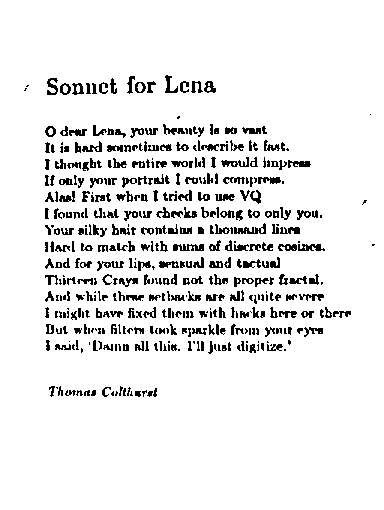
\includegraphics[width=0.5\textwidth]{src/img/p4/text_recovered.png}
        \caption{The result of text recovery}
        \label{fig:p4}
    \end{figure}
    Following is the code:
    \begin{minted}{python}
import cv2
import os
import numpy as np

os.makedirs("result/p4", exist_ok=True)

img = cv2.imread("src/Fig3.GIF", cv2.IMREAD_GRAYSCALE)
if img is None:
    raise FileNotFoundError("Cannot open Fig3.GIF")

clahe = cv2.createCLAHE(clipLimit=2.0, tileGridSize=(8,8))
img_eq = clahe.apply(img)

"""A good result is obtained with block size = 25 and C = 10."""
binary = cv2.adaptiveThreshold(img_eq, 255,
                               cv2.ADAPTIVE_THRESH_GAUSSIAN_C,
                               cv2.THRESH_BINARY,
                               25, 10)
cv2.imwrite("result/p4/text_recovered.bmp", binary)

print("Saved result to result/p4/text_recovered.bmp")
    \end{minted}
    As the picture shows, though most of the noise is removed, but the result of the text recovery is still not very good. Some of the text structures are broken. To address this, I tried to train a Denoisy UNet to further improve the image quality.
    
    \textbf{$\boxed{\text{Denoisy UNet: }}$}
    If you are interested in the code of Denoisy UNet, you can find it at \url{https://github.com/W-X-Dai/text_recovery}. 
    
    For the training data, I generated 20000 clean samples, each sample contains a white background with black text. Then, I added Gaussian noise and illumination gradient to these clean samples to create noisy samples. Finally, I use my code in this homework to simulate the result of CLAHE and adaptive thresholding, and use these processed images as the input of the Denoisy UNet. Fig.~\ref{fig:p4_noisy} is an example of noisy data:
    \begin{figure}[H]
        \centering
        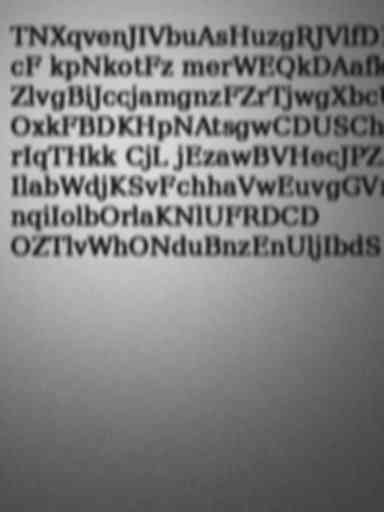
\includegraphics[width=0.5\textwidth]{src/img/noisy.png}
        \caption{An example of the noisy data}
        \label{fig:p4_noisy}
    \end{figure}


    And Fig.~\ref{fig:p4_data} is an example of the train result after 100 epochs: (Left is the broken input, middle is the output of the Denoisy UNet, right is the ground truth)
    \begin{figure}[H]
        \centering
        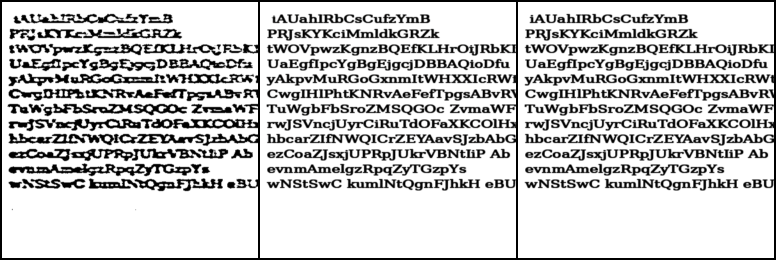
\includegraphics[width=0.9\textwidth]{src/img/dunet.png}
        \caption{An example of the training data}
        \label{fig:p4_data}
    \end{figure}
    
    Then I applied this model to the result of CLAHE and adaptive thresholding, and got the final result shown in Fig.~\ref{fig:p4_final}:
    \begin{figure}[H]
        \centering
        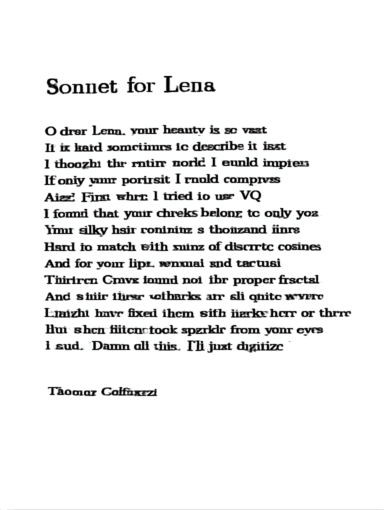
\includegraphics[width=0.5\textwidth]{src/img/p4_final.png}
        \caption{The final result after using Denoisy UNet}
        \label{fig:p4_final}
    \end{figure}
    
    \end{enumerate}
\end{document}